\section{Ergebnisse und Berechnungen}
\label{sec:ergebnisse}

In Tab. \ref{tab:ergebnisse} sind die Messdaten des Versuches dargestellt. Auf den Seiten 6 bis 11 wird eine Beispielrechnung für eine Strömungsgeschwindigkeit von Luft in einem Rohr erläutert. Die restlichen Berechnungsergebnisse sind der Tab. \ref{tab:berechnung} aufgeführt.
% Table generated by Excel2LaTeX from sheet 'Daten'
\begin{table}[h!]
	\centering
	\renewcommand{\arraystretch}{1.2}
	\caption{gut gefälschte Volumenströme und Temperaturen der verschiedenen Rohre für Wasser und Luft}
	\resizebox{16cm}{!}{
	\begin{tabular}{l|rrrrr|rrrrr|rrrrr}
		\hline
		\multicolumn{1}{r}{} & \multicolumn{5}{c}{WÜ 1}            & \multicolumn{5}{c}{WÜ 4}            & \multicolumn{5}{c}{WÜ6} \\
		\midrule
		\textbf{Messwert} & \multicolumn{1}{l}{\textbf{M11}} & \multicolumn{1}{l}{\textbf{M12}} & \multicolumn{1}{l}{\textbf{M13 }} & \multicolumn{1}{l}{\textbf{M14}} & \multicolumn{1}{l|}{\textbf{M15}} & \multicolumn{1}{l}{\textbf{M41}} & \multicolumn{1}{l}{\textbf{M42}} & \multicolumn{1}{l}{\textbf{M43}} & \multicolumn{1}{l}{\textbf{M44}} & \multicolumn{1}{l|}{\textbf{M45}} & \multicolumn{1}{l}{\textbf{M61}} & \multicolumn{1}{l}{\textbf{M62}} & \multicolumn{1}{l}{\textbf{M63}} & \multicolumn{1}{l}{\textbf{M64}} & \multicolumn{1}{l}{\textbf{M65}} \\
		\midrule
		$\dot{V}_{\ce{H2O}} \, \left[\si{\liter\per\hour}\right]$   & 385   & 401   & 418   & 422   & 431   & 422   & 425   & 412   & 420   & 435   & 431   & 434   & 413   & 421   & 417 \\
		$\dot{V}_L \, \left[\si{\raiseto{3} \meter \per\hour}\right]$   & 25,5  & 11    & 19,1  & 22,1  & 16    & 25,2  & 19,9  & 15,1  & 12,3  & 10,4  & 24,9  & 19,7  & 16    & 12,1  & 9,9 \\
		$T_{\ce{H2O},\alpha} \, \left[\si{\celsius}\right]$     & \multicolumn{1}{l}{-} & \multicolumn{1}{l}{-} & \multicolumn{1}{l}{-} & \multicolumn{1}{l}{-} & \multicolumn{1}{l|}{-} & \multicolumn{1}{l}{-} & \multicolumn{1}{l}{-} & \multicolumn{1}{l}{-} & \multicolumn{1}{l}{-} & \multicolumn{1}{l|}{-} & \multicolumn{1}{l}{-} & \multicolumn{1}{l}{-} & \multicolumn{1}{l}{-} & \multicolumn{1}{l}{-} & \multicolumn{1}{l}{-} \\
		$T_{\ce{H2O},\omega} \, \left[\si{\celsius}\right]$   & 54,5  & 57    & 50,58 & 55,1  & 55,83 & 54,7  & 54,7  & 54,72 & 53,8  & 54,2  & 55,97 & 56,3  & 55,8  & 55,7  & 55,1 \\
		 $T_{\text{Luft},\alpha}\, \left[\si{\celsius}\right]$  & 24,51 & 20,41 & 20,21 & 18,09 & 17,86 & 26,42 & 24,51 & 22,81 & 21,52 & 20,53 & 20,51 & 20,4  & 20,42 & 20,39 & 20,36 \\
		$T_{\text{Luft},\omega}\, \left[\si{\celsius}\right]$   & 37,92 & 39,52 & 34,54 & 35,54 & 36,19 & 35    & 34,78 & 33,61 & 33,49 & 32,67 & 28,82 & 29,54 & 29,4  & 29,8  & 30,53 \\
		$\Delta p \ \left[\si{\mmWS}\right]$    & 0     & 0     & 0     & 0     & 0     & 0     & 0     & 0     & 0     & 0     & 0     & 0     & 0     & 0     & 0 \\
		\bottomrule
	\end{tabular}}
	\label{tab:ergebnisse}%
\end{table}%
\FloatBarrier

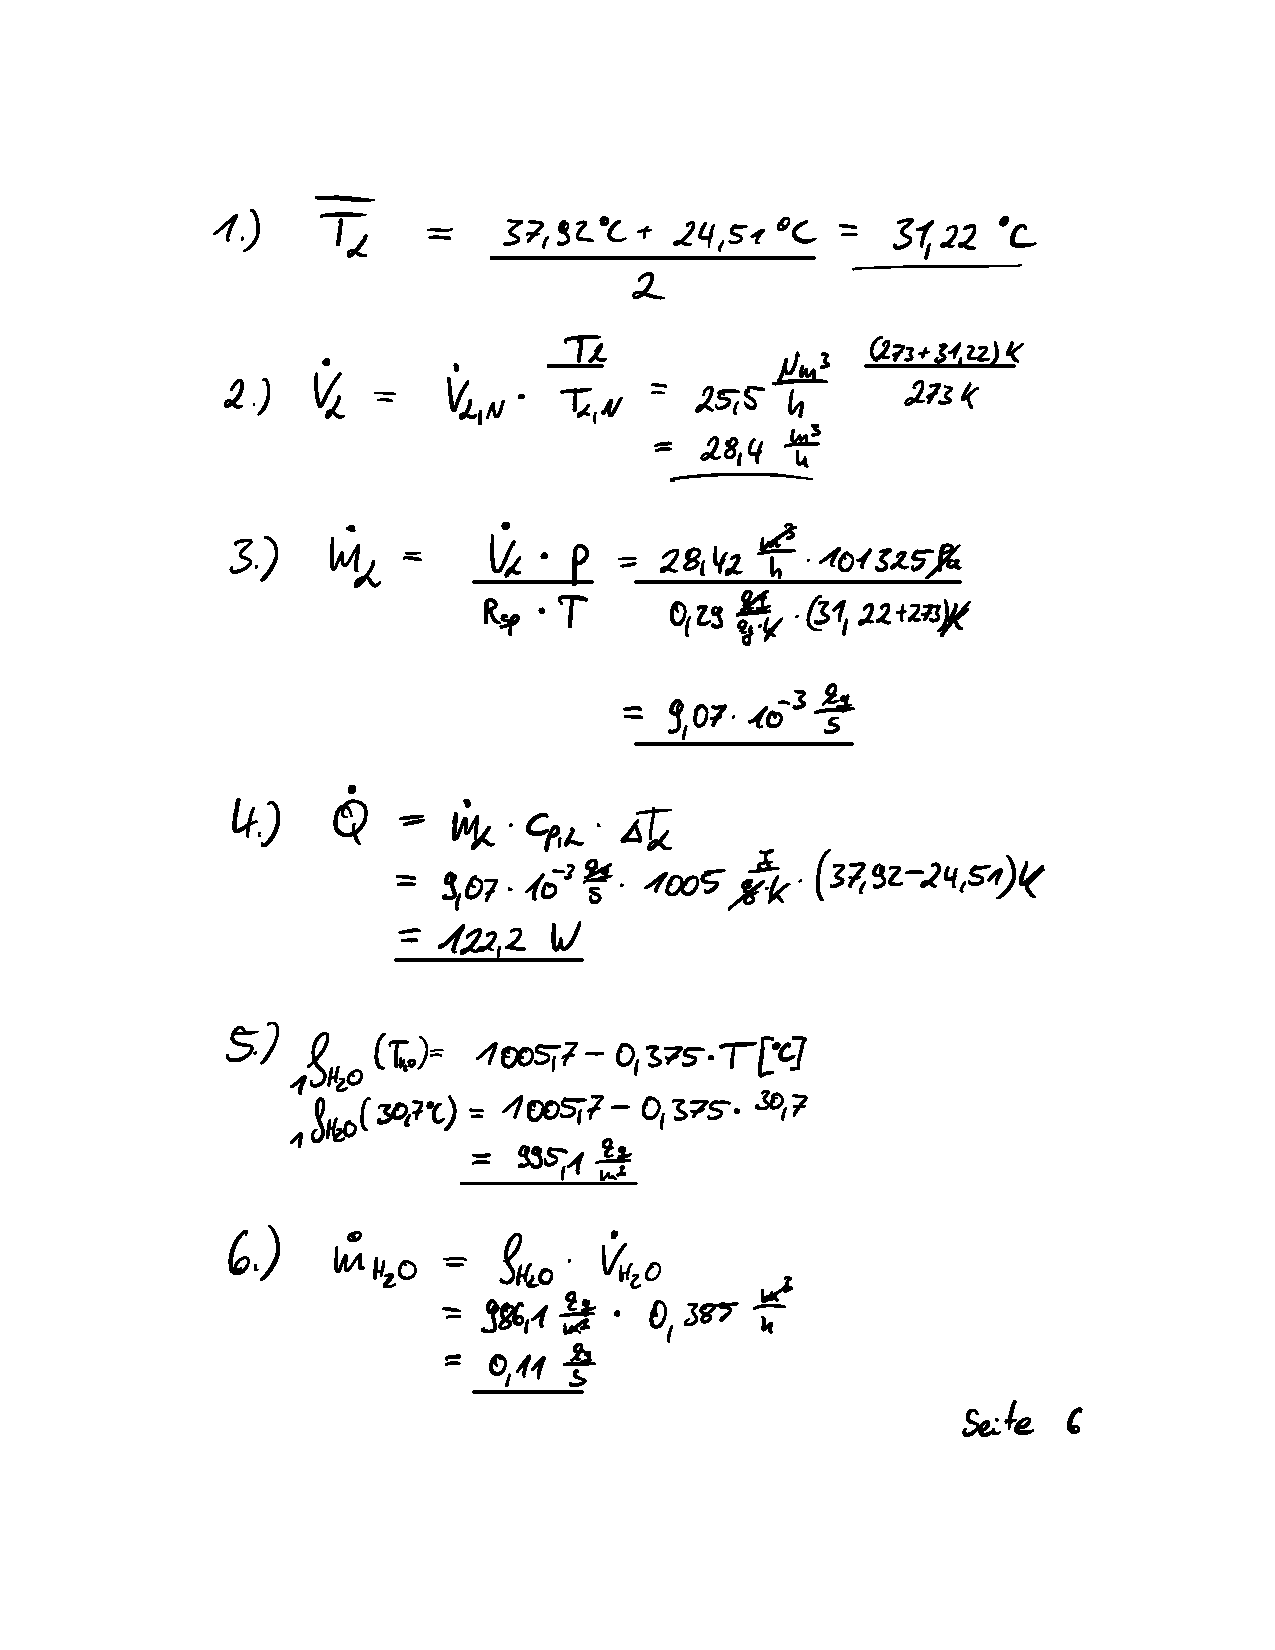
\includepdf[pages=1-6]{data/Beispielrechnung2.pdf}


\begin{sidewaystable}[h!]
		\centering
		\renewcommand{\arraystretch}{1.2}
		\caption{Berechnete Daten der Wärmeübertrager}
		\resizebox{25cm}{!}{
		\begin{tabular}{l|rrrrr|rrrrr|rrrrr}
			\hline
			\multicolumn{1}{c|}{\textbf{Messwert}} & \multicolumn{1}{c}{M11} & \multicolumn{1}{c}{M12} & \multicolumn{1}{c}{M13} & \multicolumn{1}{c}{M14} & \multicolumn{1}{c|}{M15} & \multicolumn{1}{c}{M41} & \multicolumn{1}{c}{M42} & \multicolumn{1}{c}{M43} & \multicolumn{1}{c}{M44} & \multicolumn{1}{c|}{M45} & \multicolumn{1}{c}{M61} & \multicolumn{1}{c}{M62} & \multicolumn{1}{c}{M63} & \multicolumn{1}{c}{M64} & \multicolumn{1}{c|}{M65} \\
			\hline
			$\dot{V}_L \, \left[\si{\raiseto{3} \meter \per \hour}\right]$& 28,42 & 12,21 & 21,02 & 24,27 & 17,58 & 28,03 & 22,06 & 16,66 & 13,54 & 11,41 & 27,15 & 21,50 & 17,46 & 13,21 & 10,82 \\
			$\dot{V}_{\ce{H2O}}\, \left[\si{\raiseto{3} \meter \per \hour}\right]$ & 0,39  & 0,40  & 0,42  & 0,42  & 0,43  & 0,42  & 0,43  & 0,41  & 0,42  & 0,44  & 0,43  & 0,43  & 0,41  & 0,42  & 0,42 \\
			$\overline{T_L} \, \left[\si{\celsius}\right]$ & 54,64 & 57,08 & 50,68 & 55,24 & 55,94 & 54,78 & 54,77 & 54,78 & 53,85 & 55,87 & 56,04 & 56,36 & 55,85 & 55,74 & 55,14 \\
			$\rho_{\ce{H2O}} \, \left[\si{\kg\per\raiseto{3}\meter}\right]$ & 986,10 & 984,94 & 987,88 & 985,82 & 985,49 & 986,03 & 986,03 & 986,03 & 986,46 & 985,52 & 985,44 & 985,29 & 995,08 & 985,58 & 985,87 \\
			$\rho_L \, \left[\si{\kg\per\raiseto{3}\meter}\right]$& 1,15  & 1,15  & 1,16  & 1,17  & 1,16  & 1,15  & 1,15  & 1,16  & 1,16  & 1,17  & 1,17  & 1,17  & 1,17  & 1,17  & 1,17 \\
			$\dot{m_L} \, \left[\si{\kg\per\second}\right]$& 9,07E-03 & 3,91E-03 & 6,79E-03 & 7,86E-03 & 5,69E-03 & 8,96E-03 & 7,07E-03 & 5,37E-03 & 4,37E-03 & 3,70E-03 & 8,85E-03 & 7,00E-03 & 5,69E-03 & 4,30E-03 & 3,52E-03 \\
			$\dot{m_{\ce{H2O}}} \, \left[\si{\kg\per\second}\right]$& 0,11  & 0,11  & 0,12  & 0,12  & 0,12  & 0,12  & 0,12  & 0,11  & 0,12  & 0,12  & 0,12  & 0,12  & 0,11  & 0,12  & 0,12 \\
			$\dot{Q} \, \left[\si{\watt}\right]$ & 122,18 & 75,11 & 97,79 & 137,79 & 104,79 & 77,25 & 73,02 & 58,27 & 52,60 & 45,11 & 73,93 & 64,33 & 51,34 & 40,68 & 35,97 \\
			$\Delta T_{\ce{H2O}} \, \left[\si{\kelvin}\right]$& 0,27  & 0,16  & 0,20  & 0,28  & 0,21  & 0,16  & 0,15  & 0,12  & 0,11  & 0,09  & 0,15  & 0,13  & 0,11  & 0,08  & 0,07 \\
			$ T_{\ce{H2O},\alpha }\, \left[\si{\kelvin}\right]$ & 54,77 & 57,16 & 50,78 & 55,38 & 56,04 & 54,86 & 54,85 & 54,84 & 53,91 & 55,92 & 56,12 & 56,43 & 55,91 & 55,78 & 55,17 \\
			$\overline{T}_{\ce{H2O}} \, \left[\si{\kelvin}\right]$ & 54,64 & 57,08 & 50,68 & 55,24 & 55,94 & 54,78 & 54,77 & 54,78 & 53,85 & 55,87 & 56,04 & 56,36 & 55,85 & 55,74 & 55,14 \\
			$LNTD \, \left[\si{\kelvin}\right]$ & 22,79 & 25,97 & 22,57 & 27,54 & 27,94 & 23,82 & 24,79 & 26,21 & 25,90 & 28,86 & 31,20 & 31,18 & 30,73 & 30,41 & 29,40 \\
			$U_a \, \left[\si{W \per \raiseto{2}\meter \per \kelvin}\right] $& 100,12 & 54,01 & 80,92 & 93,46 & 70,06 & 38,29 & 34,78 & 26,25 & 23,98 & 18,46 & 88,52 & 77,09 & 62,41 & 49,98 & 45,71 \\
			$d_H \, \left[\si{\meter}\right] $& 8,40E-03 & 8,40E-03 & 8,40E-03 & 8,40E-03 & 8,40E-03 & 1,06E-02 & 1,06E-02 & 1,06E-02 & 1,06E-02 & 1,06E-02 & 8,40E-03 & 8,40E-03 & 8,40E-03 & 8,40E-03 & 8,40E-03 \\
			$A_{\ce{H2O}} \, \left[\si{\raiseto{2} \meter}\right]$ & 3,36E-04 & 3,36E-04 & 3,36E-04 & 3,36E-04 & 3,36E-04 & 6,49E-04 & 6,49E-04 & 6,49E-04 & 6,49E-04 & 6,49E-04 & 3,36E-04 & 3,36E-04 & 3,36E-04 & 3,36E-04 & 3,36E-04 \\
			$w_{\ce{H2O}} \, \left[\si{\meter\per\second}\right]$ & 0,32  & 0,33  & 0,35  & 0,35  & 0,36  & 0,18  & 0,18  & 0,18  & 0,18  & 0,19  & 0,36  & 0,36  & 0,34  & 0,35  & 0,34 \\
			$Re_{\ce{H2O}} \, \left[-\right]$ & 5,22E+03 & 5,65E+03 & 5,32E+03 & 5,78E+03 & 5,96E+03 & 3,75E+03 & 3,78E+03 & 3,66E+03 & 3,68E+03 & 3,93E+03 & 5,97E+03 & 6,05E+03 & 5,71E+03 & 5,81E+03 & 5,70E+03 \\
			$Pr_{\ce{H2O}} \, \left[-\right]$& 3,27  & 3,13  & 3,51  & 3,23  & 3,19  & 3,26  & 3,26  & 3,26  & 3,31  & 3,19  & 3,18  & 3,17  & 3,23  & 5,34  & 3,24 \\
			$Nu_{\ce{H2O}} \, \left[-\right]$& 34,79 & 36,42 & 36,34 & 37,57 & 38,35 & 26,67 & 26,83 & 26,17 & 26,44 & 27,49 & 38,37 & 38,65 & 37,19 & 46,13 & 37,19 \\
			$\alpha_{\ce{H2O},a} \, \left[\si{\watt\per\raiseto{2}\meter\per\kelvin}\right]$ & 2677  & 2814  & 2777  & 2893  & 2957  & 1627  & 1636  & 1596  & 1610  & 1680  & 2959  & 2982  & 2867  & 3556  & 2864 \\
			$d_i \, \left[\si{\meter}\right]$ & 1,73E-02 & 1,73E-02 & 1,73E-02 & 1,73E-02 & 1,73E-02 & 2,97E-02 & 2,97E-02 & 2,97E-02 & 2,97E-02 & 2,97E-02 & 1,73E-02 & 1,73E-02 & 1,73E-02 & 1,73E-02 & 1,73E-02 \\
			$A_{L} \, \left[\si{\raiseto{2} \meter}\right]$  & 2,35E-04 & 2,35E-04 & 2,35E-04 & 2,35E-04 & 2,35E-04 & 6,93E-04 & 6,93E-04 & 6,93E-04 & 6,93E-04 & 6,93E-04 & 2,35E-04 & 2,35E-04 & 2,35E-04 & 2,35E-04 & 2,35E-04 \\
			$w_{L} \, \left[\si{\meter\per\second}\right]$ & 33,58 & 14,43 & 24,83 & 28,68 & 20,78 & 11,24 & 8,85  & 6,68  & 5,43  & 4,58  & 32,08 & 25,41 & 20,63 & 15,61 & 12,79 \\
			Re Luft [-] & 3,60E+04 & 1,56E+04 & 2,72E+04 & 3,15E+04 & 2,28E+04 & 2,07E+04 & 1,64E+04 & 1,25E+04 & 1,02E+04 & 8,65E+03 & 3,57E+04 & 2,82E+04 & 2,29E+04 & 1,73E+04 & 1,42E+04 \\
			$Pr_L \, \left[-\right]$ & 0,70  & 0,70  & 0,70  & 0,70  & 0,70  & 7,03E-01 & 7,03E-01 & 7,03E-01 & 7,03E-01 & 7,04E-01 & 7,04E-01 & 7,04E-01 & 7,04E-01 & 7,04E-01 & 7,04E-01 \\
			$\alpha_{L,i} \, \left[\si{\watt\per\raiseto{2}\meter\per\kelvin}\right]$ & 130,0 & 68,3  & 103,9 & 120,6 & 89,3  & 44,7  & 40,5  & 30,4  & 27,7  & 21,2  & 113,8 & 98,5  & 79,3  & 62,9  & 57,6 \\
			$Nu_L\, \left[-\right]$& 85    & 45    & 68    & 80    & 59    & 50    & 46    & 34    & 31    & 24    & 76    & 65    & 53    & 42    & 38 \\
			$\ln({(Re_L)}^2*Pr_L)$& 20,63 & 18,95 & 20,07 & 20,37 & 19,72 & 19,53 & 19,06 & 18,52 & 18,11 & 17,78 & 20,62 & 20,15 & 19,73 & 19,17 & 18,77 \\
			$\ln(Nu_L)$& 4,44  & 3,80  & 4,23  & 4,38  & 4,08  & 3,92  & 3,82  & 3,54  & 3,45  & 3,18  & 4,33  & 4,18  & 3,96  & 3,73  & 3,64 \\
		  \end{tabular}
		}
	\label{tab:berechnung}
\end{sidewaystable}
\FloatBarrier	

Um die verschiedenen Wärmetauscher vergleichen zu können und ein Optimum für den Betrieb des Wärmetauschers zu verfolgen, wird eine Linearisierung der \textsc{Nußelt}-Gleichung mit den Parametern $a$ und $b$ vorgenommen (siehe Gl.\eqref{gl:linearisierung}).
Diese werden für die verschiedenen Versuchsbedingungen und Wärmetauscher im Diagramm Abb. \ref{dia:nusselt} aufgetragen.

\begin{flalign}
\label{gl:linearisierung}
\tag{Geradengleichung} y 	&= m*x + n\\
\tag{logarithmieren}
Nu 	&= a*\left(Re^2*Pr\right)^b\\
\ln(Nu) 	&= \ln(a)+b*\ln(Re^2*Pr)
\end{flalign}

\begin{figure}[h!]
		\begin{center}
			\resizebox{0.8\textwidth}{!}{
				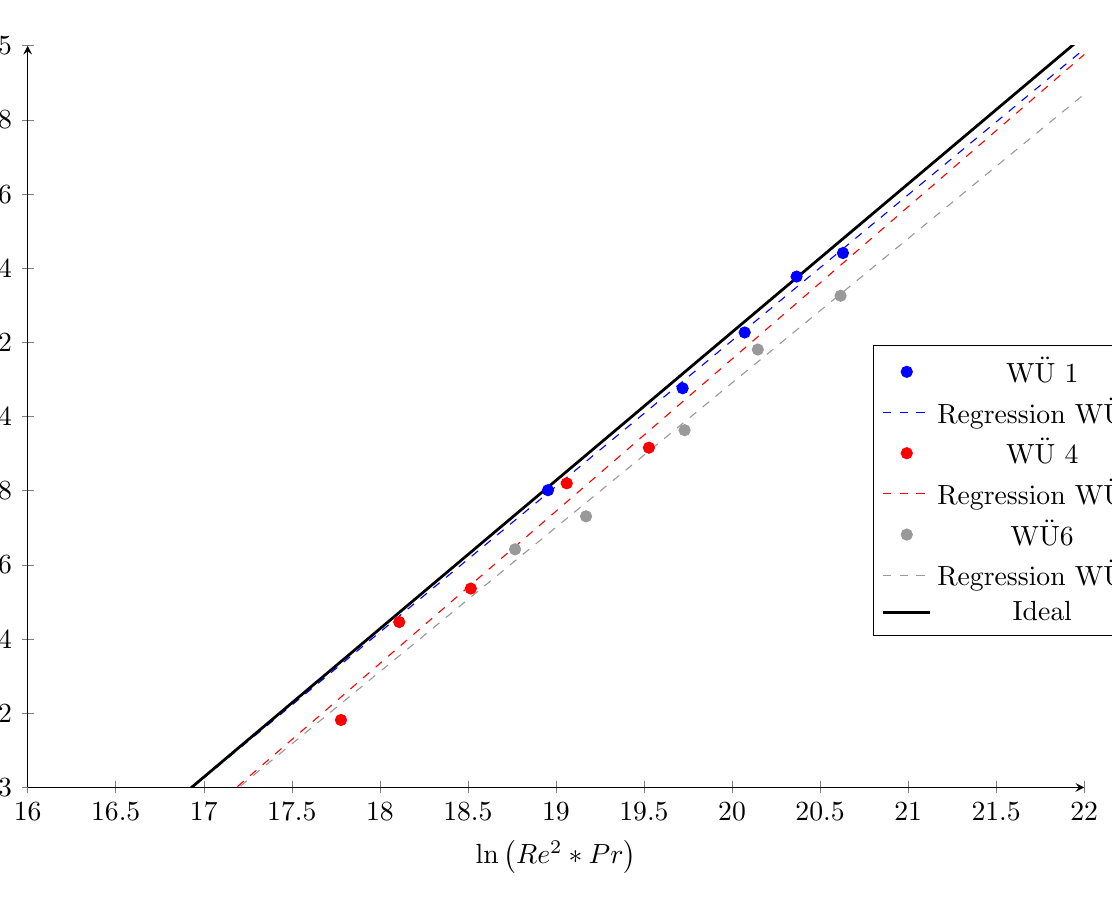
\begin{tikzpicture}[trim axis left, trim axis right]
				\begin{axis}[
				axis lines = left,
				width = 15cm,
				height = 11cm,
				xmin = 16,
				xmax = 22,
				ymin = 3,
				ymax = 5,
				%	ytick = {-4.5,-4,...,-1},
				%	xtick = {-10,-9,...,20},
				ylabel={$\ln(Nu)=\ln(a)$},
				%y label style={at={(0,0.5)}},
				xlabel={$\ln\left(Re^2*Pr\right)$},
				legend style={at={(0.8,0.4)},anchor=west},
				%	y dir = reverse,
				]
				\addplot [color=blue, mark=*, only marks] coordinates{(20.6297374908074,4.44104369234906) (18.9546273718935,3.80144109711371) (20.0716652877696,4.22683350226042) (20.3663656925989,4.37753401861674) (19.7192916621653,4.07642094111326) };
				
				\addplot +[mark=none, dashed, blue, domain=0:25] {x*0.393184906-3.658730546};
				
				
				\addplot [color=red, mark=*, only marks] coordinates{(19.5277930158006,3.91608551420758) (19.0610517373774,3.82007146704219) (18.5164491828898,3.53620711030527) (18.1099284493333,3.44591529294571) (17.7790640575647,3.18172509942449) };
				
				\addplot +[mark=none, dashed, red, domain=0:25] {x*0.410555238-4.055857385};
				
				\addplot [color=black!40!white, mark=*, only marks] coordinates{(20.6162086982967,4.32579265627852) (20.1461082909801,4.18077187238098) (19.7303635113762,3.9632873963571) (19.1706257554954,3.73097328400248) (18.7674483798004,3.64195918704045)  };
				
				\addplot +[mark=none, dashed, color=black!40!white, domain=0:25] {x*0.389412718-3.697480663};
								
				\addplot [color=black, mark=none,line width=1.pt ] coordinates{	(10,0.227738936947013) (10.5,0.427738936947013) (11,0.627738936947013) (11.5,0.827738936947013) (12,1.02773893694701) (12.5,1.22773893694701) (13,1.42773893694701) (13.5,1.62773893694701) (14,1.82773893694701) (14.5,2.02773893694701) (15,2.22773893694701) (15.5,2.42773893694701) (16,2.62773893694701) (16.5,2.82773893694701) (17,3.02773893694701) (17.5,3.22773893694701) (18,3.42773893694701) (18.5,3.62773893694701) (19,3.82773893694701) (19.5,4.02773893694701) (20,4.22773893694701) (20.5,4.42773893694701) (21,4.62773893694701) (21.5,4.82773893694701) (22,5.02773893694701) (22.5,5.22773893694701) (23,5.42773893694701) (23.5,5.62773893694701) (24,5.82773893694701) (24.5,6.02773893694701) (25,6.22773893694701) (25.5,6.42773893694701) (26,6.62773893694701) (26.5,6.82773893694701) (27,7.02773893694701) (27.5,7.22773893694701) (28,7.42773893694701)  };
				
				\legend{WÜ 1, Regression WÜ 1, WÜ 4, Regression WÜ 4, WÜ6, Regression WÜ 6, Ideal}
				\end{axis}
				\end{tikzpicture}
			}
			\caption{linearisierte \textsc{Nußelt}-Gleichung in Abhängigkeit von $Re$, $Pr$, $a$ und $b$}
			\label{dia:nusselt}
		\end{center}
	\end{figure}
	\FloatBarrier
\begin{table}[h!]
	\centering
	\caption{\textsc{Nußelt}-Koeffizienten $a$ und $b$ bestimmt aus Abb. \ref{dia:nusselt} mittels Anstieg $b$ und Achsenabschnitt $\ln(a)$}
	\label{tab:ab}
		%\resizebox{10.5cm}{!}{
			\begin{tabulary}{1.0\textwidth}{C|CCC|C}
				\textbf{} & \textbf{WÜ 1} & \textbf{WÜ 4}&\textbf{WÜ 6}&\textbf{Ideal}\\
				\hline
				$\ln(a)$&-3,66&-4,06&-3,70&-3,77\\
				$a$ & 0,026&0,017&0,025&0,023\\
				$b$ &0,39&0,41&0,39&0,4\\
				\hline
				$R^2$&0,929&0,968&0,827&1,000\\
				\hline		
	\end{tabulary}
%}
\end{table}%
\FloatBarrier

Das Bestimmtheitsmaß Daten in Tab. \ref{tab:ab} gibt an, dass $R^2$ zwischen $0,827$ und $0,968$ liegt. Dadurch sind starke Abweichungen zu erkennen, die im Präsenspraktikum zumindest für WÜ 6 wiederholt werden sollte.
Ansonsten lässt sich aus Abb. \ref{dia:nusselt} erkennen, dass die Regressionsgeraden von WÜ 1 am nächsten an der idealen Geraden anliegt.
